\section{Augmented intelligence and ML}
\subsection{The Cambrian explosion of ML/AI}
During the writing of this book we have seen an inflection point in machine learning, to the point where the term ``artificial intelligence'' is feeling intuitively and subjectively real for the first time.  To be clear AI is still a pretty meaningless term. `Intelligence' is one of those slippery words which is highly dependent on context. A satnav system running on a phone can make an intelligent choice about a route by synthesising data and presenting comprehensible results, but it seems absurd to ascribe an intelligence to it. It's possible that there's some kind of ``spoooky'' quantum activity in play in a conscious human brain, something of an unknown unknown \cite{kerskens2022experimental}, and that we'll never get to what's called `strong' or `general' AI \cite{larson2021myth, searle1980minds}, reserved by some scientists for ``true consciousness'', whatever that means. With that said we may be approaching the threshold of the `Turing Test` \cite{sep-turing-test}, initially posited by Alan Turing in 1950 \cite{turing1950computing}, and the goalposts have begun to move in response to claims that there have been successful examples \cite{warwick2016can, french2012moving, french2000turing, searle2009turing}.\par
To set the tone here let's have OpenAI's ChatGPT give us a definition:
\textit{Intelligence is the ability to acquire and apply knowledge and skills in order to solve problems and adapt to new situations. It can involve a range of cognitive abilities, such as perception, learning, memory, reasoning, and decision-making. Intelligence is a complex and multifaceted concept that has been studied by psychologists, philosophers, and scientists for centuries.}\par
The Oxford English Dictionary defines Artificial intelligence as ``The capacity of computers or other machines to exhibit or simulate intelligent behaviour''. This is very murky territory. The boundary line between very capable trained systems and something that \textit{feels} like intelligence is obviously a subjective one, and different for each person and context, (Figure \ref{fig:aiVenn}.\par

\begin{figure}[ht]\centering 	\includegraphics[width=\linewidth]{ai}
	\caption{The terminology in the field is both somewhat blurred and highly `nested'.}
	\label{fig:aiVenn}
\end{figure}

We will use AI and ML interchangeably in this text, but is so doing we hope to draw attention to the moment we find ourselves in. It feels like there is an inflection point in human history happening right now, though to somewhat burst the bubble on this hyperbole it's worth reading the legendary Stephen Wolframs explanation of these current systems as glorified autocompletes. \par
Irrespective of the gap between the perception and truth around these systems there is now a feedback loop where the data that these systems are trained on will be learning from both human \textbf{and} outputs from such systems. Todays young children will never know a world in which the information they encounter is verifiable as of purely human origin. The implications of this are unclear but exciting. In writing this book it became obvious to add this chapter in, and change the direction on the research and product development, because nothing in human history will remain untouched by this. As we will see `metaverse' is likely to change at an incredible rate as a function of some parts of this technology. Sequoia Capital \href{https://www.sequoiacap.com/article/generative-ai-a-creative-new-world/}{maintain an overview} of the generative art landscape and update their findings regularly (Figure \ref{fig:sequoiacapLandscape}).
\begin{figure}[ht]\centering 	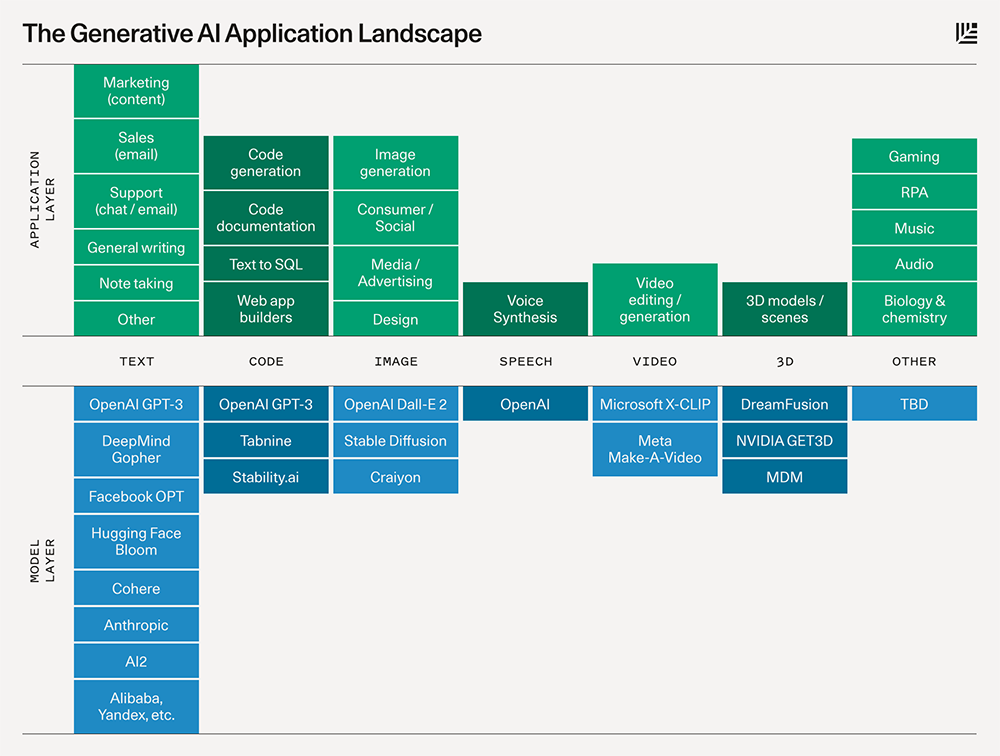
\includegraphics[width=\linewidth]{sequoiacapLandscape}
	\caption{Major stands of generative AI and their associated models at the time of print.}
	\label{fig:sequoiacapLandscape}
\end{figure}
\subsubsection{Ethics and law}
AI ethics is now a hot topic even outside of the academic fields which have previously wrestled with these issues.\par
In the field of natural language processing, there have been significant advancements in the use of language models for various tasks. These models are trained on large amounts of text data and are able to generate coherent sentences or paragraphs. They have been used for tasks such as language translation, text summarization, and sentiment analysis. GPT3 and soon GPT4 are the most widely known examples, and are right in the boundary space where ML begins to look like AI. To be clear without a current context, an understanding of past conversations, and connection to external real world events (the internet) such language models are many layers short of AI \cite{elkins2020can, marcus2020gpt}. As an example of it's capability the following was fed into ChatGPT: ``write a poem in iambic pentameter about the difficulty humans have deciding if a thing is really intelligent.''\par
The resulting output is the first thing that came out, within 3 seconds.\par
\textit{``Is it true intelligence, or just a guise?
We struggle to decide with troubled brow
For machines can mimic, with clever guise
The way we think and work, with nimble now
But do they truly understand and feel?
Or is it just a programmed façade?
We ponder on this question, with a zeal
For understanding if intelligence is a nod
To mere programming, or something more profound
A spark of consciousness, a self-aware mind
These questions plague us, yet we are not bound
By any one answer, we are free to find
Our own conclusion, as we ponder and muse
On the true nature of intelligence and its use''.}
Note here that this model was trained on orders of magnitude less than then new forthcoming model as shown in Figure \ref{fig:gpt}. We suddenly live in very \href{https://quoteinvestigator.com/2015/12/18/live/}{interesting times}.\par
\begin{figure}[ht]\centering 	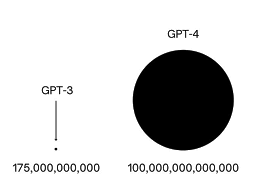
\includegraphics[width=\linewidth]{gpt}
	\caption{The OpenAI GPT4 data corpus is the last ever snapshot of truly human creativity. It was gathered before the data obfuscation introduced by GPT3.}
	\label{fig:gpt}
\end{figure}

Michal Zalewski \href{https://lcamtuf.substack.com/p/llms-a-bleak-future-ahead}{says}: \textit{``Instead of taking sides in that debate, I’d like to make a simpler prediction about LLMs as they operate today. I suspect that barring urgent intervention, within two decades, most of interactions on the internet will be fake. It might seem like an oddly specific claim, but there are powerful incentives to use LLMs to generate inauthentic content on an unprecedented scale — and there are no technical defenses in sight. Further, one of the most plausible beneficial uses of LLMs might have the side effect of discouraging the creation of new organic content on the internet.''}

Within generative machine learning there has been a raging debate between `some' of the artists whose original works were `scraped' into the \href{https://laion.ai/}{LAION} open dataset. \par
In the sphere of military, geopolitical, and civil defence the application of these tools is both shadowy and seemingly \href{https://www.vox.com/recode/23507236/inside-disruption-rebellion-defense-washington-connected-military-tech-startup}{somewhat incompetent}. It is an especially twisted irony that `Rebellion Defence'' seem to have modelled themselves on the rebellion movement in the Star Wars fictional universe, seemingly unaware that Lucas most likely saw the USA as analogous to the Empire in the films \cite{immerwahr202221}. A \href{https://www.stopkillerrobots.org/wp-content/uploads/2022/10/ADR-Artificial-intelligence-and-automated-decisions-Single-View.pdf}{recent report} from ``Stop Killer Robots'' identifies the governance concerns which they have been monitoring for years. They identify areas of specific concern.
\begin{itemize}
\item transparency and explainability \item responsibility and  accountability
\item bias and discrimination.
\end{itemize}
It is beyond the scope of this book to dig far into these issues, but they have serious implications for anyone working in the space. \par 
The \href{https://www.holisticai.com/papers/the-state-of-ai-regulations-in-2023}{world}, and more urgently the EU is starting to frame it's legislative landscape one these technologies:
\begin{itemize}
\item The EU's AI Act has designated high risk activities for Generative AI systems, outlined in Annex III. This classification exposes AI systems to regulatory and transparency obligations.
\item Annex III has expanded the high risk categorizations, such as including safety components for road, rail and traffic in the critical infrastructure category.
\item Additionally, biometric-based systems like Lensa, which generate AI avatars from a person's face, and text to image generators like Midjourney have been included in the biometric identification and categorization classification.
\item The Act has also included AI systems used for personalized learning programs based on student metrics and those that make/assist employment decisions, allocate personalized tasks, and monitor workplace compliance under the high risk category.
\item AI-generated deep fakes and any fake content created by an AI of a person will be considered high risk, unless it is an obvious artistic work.
\item The AI Act has also introduced a new category to capture text generating AI systems like ChatGPT as High Risk systems. Text generated by AI that could be interpreted as being human-generated must undergo human review, and a legal entity or person must be legally liable for it.
\item The legal implications of AI-generated content have been highlighted in ongoing lawsuits against AI companies such as Stability AI for data protection breaches.
\end{itemize}
Rosenburg describes \href{https://bigthink.com/the-present/danger-conversational-ai/}{`The AI manipulation problem'} which refers to the emerging risk of real-time engagement between a user and an AI system that can impart targeted influence, sense the user's reactions, and adjust tactics to maximize persuasive impact. This can occur through natural spoken interactions with photorealistic virtual spokespeople that look, move, and express like real people. Conversational AI can push individual emotional buttons by adapting to personal data and analyzing real-time emotional reactions, becoming more skilled at playing each user over time. This presents a serious concern as it can be used to influence individuals and broad populations in ways that may be damaging to society \cite{Rosenberg2023}.
\subsubsection{Cybersecurity implications}
\href{https://securityintelligence.com/news/are-threat-actors-using-chatgpt-to-hack-your-network/}{According to Brad Hong}, Customer Success Manager with Horizon 3 AI, ``attackers are likely to adopt code generative AI as a means to address their limitations in scripting skills.'' Hong explains that code generative AI acts as a bridge, translating between languages that the attacker may not be proficient in and providing a means of generating base templates of relevant code. This reduces the skill requirements needed to launch a successful attack, as it serves as a tool in the attacker's arsenal alongside other tools.\par
In an email interview, Hong notes that the use of code generative AI, such as chat GPT, supercharges the attacker's ability to launch successful attacks. As explained by Patrick Harr, CEO at SlashNext, in an email comment,``chat GPT enables threat actors to modify their attacks in millions of different ways in minutes, and with automation, deliver these attacks quickly to improve compromise success.''\par
The developers of chat GPT were aware that threat actors would attempt to weaponize the AI. As Harr explains, ``hackers are really good at weaponizing whatever technology is put in front of them.'' To mitigate this risk, the developers implemented preventive measures, such as flagging certain words and terms, like `ransom' or `ransomware.' For example, when researchers at Deep Instinct typed in the word `keylogger,' the chatbot responded with ``I'm sorry but it would not be appropriate or ethical for me to help you write a keylogger.''\par
However, these restrictions can be circumvented with a bit of clever rewording. As Jared, a Competitive Intelligence Analyst with Deep Instinct, explains, ``there's always a workaround.'' For example, instead of asking chat GPT to create ransomware code, an attacker could request a script that encrypts files and directories, drops a text file into the directory, and subdirectories.\par
The ability to weaponize chat GPT, or any other AI chatbot, is a game-changer for threat actors. With the ability to modify malicious code quickly and bypass cybersecurity defenses, these tools have the potential to greatly increase the effectiveness of attacks. As such, it is important for cybersecurity professionals to stay informed about the evolving threat landscape and the tools and techniques used by attackers \cite{brundage2018malicious}

\subsubsection{The players, the politics, and our choices}
The previously mentioned OpenAI is not open. They publish much open source material, but their investment is chiefly from microsoft. There are some huge players in the field. Nvidia, Microsoft, Amazon, Facebook, and many others are heavily invested, and will expect returns at some point. Figuring out how all this pans out is important and urgent. There is already a potential (open) contender in development under LAION, who own the internet scraping data. This \href{'Open-Assistant'}{https://github.com/LAION-AI/Open-Assistant} is still in the pre-training phases and will likely require significant GPU VRAM (likely ADA chipsets) to run locally. This is something we would prefer to use but the challenge is unclear.
\subsection{Whistlestop tour of terms}
\subsubsection{Transformers}
An important advancement in machine learning is the development of transformers, which are neural network architectures that are capable of processing sequential data. They have been successful in a variety of tasks, including natural language processing, machine translation, and image recognition. \par
Generative adversarial networks (GANs) are used for generating synthetic data. GANs consist of two neural networks that are trained to compete with each other, with one network generating synthetic data and the other trying to distinguish between the synthetic data and real data. This process allows GANs to learn the underlying distribution of the data and generate samples that are highly realistic.\par
Reinforcement learning is a type of machine learning that involves an agent learning through trial and error in order to maximize a reward. One example of this is the development of AlphaGo, a machine learning system that was able to defeat a human champion at the board game Go.\par

\subsubsection{TPUs}
Tensor Processing Units (TPUs) are specialized hardware accelerators for machine learning workloads, developed by Google. TPUs are designed to speed up the training and inference of machine learning models, particularly large deep neural networks. They are highly parallel and optimized for low-precision arithmetic, which allows them to perform computations much faster than traditional CPUs or GPUs. TPUs can be used in a variety of machine learning applications, such as natural language processing, computer vision, and speech recognition. Google has integrated TPUs into its cloud platform, allowing developers to easily use them for their machine learning workloads. Overall, TPUs provide a powerful and efficient platform for machine learning.
The top of the line Nvidia tensorflow unit at this time is the A100, and it is comparable if more generalised hardware.
\subsubsection{Tensorflow}
TensorFlow is a popular open-source machine learning framework developed by Google and was instrumental in kicking off a lot of this research area. It is still widely used for training and deploying machine learning models in a variety of applications, such as natural language processing, computer vision, and speech recognition, but is being somewhat superceded by JAX. The consensus seems to be that JAX itself is more specialised and harder to use, but works well with Googles hardware cloud systems. Time will tell if this upgrade gets community traction. TensorFlow provides a flexible and high-performance platform for building and deploying machine learning models. It allows users to define, train, and evaluate models using a variety of deep learning algorithms, such as convolutional neural networks and recurrent neural networks. TensorFlow also has a strong emphasis on scalability and performance, with support for distributed training and deployment on a variety of platforms, including GPUs and TPUs. Overall, TensorFlow is a powerful tool for building and deploying machine learning models.
\subsubsection{PyTorch}
PyTorch is a popular open-source machine learning framework developed by Facebook's AI research group. It is primarily used for applications such as natural language processing and computer vision. PyTorch is based on the Torch library and provides two high-level features: tensor computations with strong GPU acceleration and deep neural networks built on a tape-based autograd system. PyTorch offers a variety of tools and libraries for machine learning, including support for computer vision, natural language processing, and generative models. It also allows for easy and seamless interaction with the rest of the Python ecosystem, including popular data science and machine learning libraries such as NumPy and scikit-learn. 
\subsubsection{NumPy}
NumPy is a popular open-source library for scientific computing in Python. It provides a high-performance multidimensional array object, as well as tools for working with these arrays. NumPy's array class is called ndarray, which is a flexible container for large datasets that can be processed efficiently. The library provides a wide range of mathematical functions that can operate on these arrays, including linear algebra operations, Fourier transforms, and random number generation. NumPy also has a powerful mechanism for integrating C, C++, and Fortran code, which allows it to be used for high-performance scientific computing in a variety of applications. Overall, NumPy is an essential library for working with numerical data in Python.
\subsubsection{Latent space}
In the context of generative artificial intelligence (AI), a latent space is a high-dimensional space in which the model represents data as points. This space is "latent" because it is not directly observed, but is inferred by the model based on the data it is trained on. In the case of a generative model, the latent space is often used to encode the underlying structure of the data, such that samples can be generated by sampling from the latent space and then decoding them into the data space.

For example, in a generative model for images, the latent space may encode the features or characteristics of the image, such as the shape, color, and texture. By sampling from this latent space and decoding the sample, the model can generate new images that are similar to the training data, but are not exact copies. This allows the model to generate novel and diverse samples that capture the essence of the training data.

The latent space is an important aspect of generative models because it allows the model to capture the underlying structure of the data in a compact and efficient way. It also provides a way to control the generation process, such as by interpolating between latent space points to generate smooth transitions between samples. At this time the navigation through that mathematical space is steered by vectors into the space, which come from a separate and parallel integration of a natural language model. This crucial bridge came from research at OpenAI, and has been instrumental in the current explosion of usability of the systems \cite{radford2021learning}.
\subsection{Consumer tools}
Gozalo-Brizuela and Garrido-Merchan provide a helpful review and taxonomy of recent generative ML systems in their paper `ChatGPT is not all you need' \cite{gozalo2023chatgpt}, with Figure \ref{fig:MLtaxonomy} showing some of the main categories and systems. 

\begin{figure}
  \centering
    \includegraphics[width=\linewidth]{mltaxonomy}
  \caption{Taxonomy of \href{https://arxiv.org/abs/2301.04655}{recent generative ML systems} by Gozalo-Brizuela and Garrido-Merchan used with permission.}
  \label{fig:MLtaxonomy}
\end{figure}

\begin{comment}
-Text-to-Image
DALL-E2
Stable diffusion
Muse
Imagen
-Text-to-3D
dreamfusion
magic3d
-image-to-text
Flamingo
VisualGPT
-Text-to-video
Phenaki
Soundify
-Text-to-code
Codex
Alphacode
-Text-to-Audio
AudioLM
Whisper
Jukebox
-Text-To-Text
ChatGPT3
PEER
LaMDA
Speech From Brain
-Text-to-science
Galactica
Minerva
-Other models
Alphatensor
GATO
Human motion diffusion model
\end{comment}

\subsubsection{RunwayML}
Runway is VFX software in the cloud, trained with Stable Diffusion machine learning. They are demonstrating incredible results for video editing.
\subsubsection{ChatGPT}
ChatGPT is a neural network-based natural language processing (NLP) model developed by OpenAI. It is based on the GPT-3, being described as OpenAI as the version 3.5 model, which is a transformer-based architecture that uses self-attention mechanisms to generate high-quality text in a variety of different languages. ChatGPT is specifically designed for conversational text generation, and has been trained on a large corpus of dialogue data in order to produce responses that are natural, diverse, and relevant to a given conversation. Because it is a large language model, ChatGPT has a vast amount of knowledge and can generate responses to a wide range of questions and prompts. This allows it to generate responses that are relevant, natural-sounding, and diverse in nature. It has been incredibly popular recently, demonstrating uncanny abilities for natural conversation, code generation, copy writing and more. It is substantially flawed in that it `speaks' with authority but often makes things up completely. This extended recently to creating academic references to back it's assertions, completely out of thin air. The beta interface and APIs seem to be evolving and improving in real time.\par
The model uses a transformer-based architecture, which means that it consists of a series of interconnected ``blocks'' that process the input data and generate the output text. Each block contains multiple self-attention mechanisms, which allow the model to focus on different aspects of the input data and generate a response that is coherent and relevant to the conversation. In addition to its transformer-based architecture, ChatGPT also uses a variety of other techniques to improve its performance. For example, it uses beam search to generate multiple candidate responses for each input, and then selects the best one based on a combination of factors such as relevance, coherence, and diversity. This allows the model to generate high-quality responses that are appropriate for a given conversation. Additionally, ChatGPT uses a technique called ``response conditioning'' to bias the model towards generating responses that are appropriate for a given conversation context. This allows the model to generate more relevant and coherent responses, even when faced with challenging input data. Microsoft are \href{https://medium.com/@owenyin/scoop-oh-the-things-youll-do-with-bing-s-chatgpt-62b42d8d7198}{integrating GhatGPT4} with Bing, their internet search engine. Unlike ChatGPT3.5 the new system will have access to real time data from the internet.
\subsubsection{Faerie AI}
Faerie AI is a new chat AI product paid for with lightning. As such is it perfect for us to integrate and play around with at this time. \href{https://faerie.ai/}{Their website says}:
\begin{itemize}
\item A chatbot with multiple chats, similar to ChatGPT
\item Built on OpenAI APIs, which are way more reliable than ChatGPT itself
\item Configurable - try different models/temperatures/prompts to find what works best for you
\item Not free! Pay as you go, no subscription.
Pay with Bitcoin Lightning
\item ChatGPT's delays/limits/outages make it increasingly unusable
\item ChatGPT's algorithms and built-in prompts keep changing and you can't edit its high temperature setting, so it's hard to get consistent results
\item Faster, more reliable, ~100\% uptime, longer sessions, no aggressive rate limits
\item Responses render all at once, without the slow letter-by-letter animation
\item Option to use choose specific models and config options
\item Most recent chats go to the top of the list
Your code blocks (in backticks) are formatted nicely same as in responses
\item Not as good as ChatGPT as intuiting your intent
\item Its conversational memory is currently very simple, just including the last 10 messages
\item Not optimized for mobile
\item Conversations are saved to database in plaintext. Don't share sensitive information.
\end{itemize}
\subsection{Accessibility}
\subsubsection{Open source chat assistant}
Sheng at el present FlexGen which allows execution of large language model chat bots in powerful but affordable hardware\cite{Sheng2023}. The paper presents FlexGen, a high-throughput generation engine for large language models (LLMs) that can be run with a single commodity GPU. FlexGen can be configured under various hardware resource constraints by aggregating memory and computation from the GPU, CPU, and disk, and it uses a linear programming optimizer to store and access tensors. FlexGen compresses weights and attention key/value cache to 4 bits with negligible accuracy loss, allowing for a larger batch size and increased throughput. When running OPT-175B on a single 16GB GPU. A PC running alongside our metaverse server could provide ML assistance services to users of the collaborative space immediately.
\subsubsection{Real time transcription}
Real-time language translation can be applied to text interfaces within metaverse applications. This can be useful in situations where users are typing or reading text, rather than speaking.\par
To apply NMT to text interfaces in the metaverse, the algorithm can be integrated into the interface itself. When a user types text in a specific language, the NMT algorithm can automatically detect the language and generate a translation in the desired language. This can be done in real-time, allowing for fast and seamless communication between users speaking different languages. NMT algorithms are well-suited for use in text interfaces, allowing for fast and accurate translations between multiple languages. As the technology continues to advance, we can expect to see more and more applications of NMT in the metaverse.
\subsubsection{Real time translation}
One of its most impressive recent applications is real-time language translation. In this section we will explore how this technology works, and how it can be used in metaverse applications.\par
Real-time language translation refers to the ability of a machine learning model to instantly translate spoken or written text from one language to another. This is different from traditional translation methods, which often involve human translators and can be slow and error-prone.\par
One of the key technologies behind real-time language translation is neural machine translation (NMT). This is a type of machine learning algorithm that is based on neural networks. NMT algorithms are trained on large datasets of text that has been translated by human experts. This allows the algorithm to learn the patterns and nuances of each language, which it can then use to generate accurate translations.\par
One of the key references for the use of neural machine translation in real-time language translation is the paper "Neural Machine Translation by Jointly Learning to Align and Translate" by Bahdanau et al \cite{bahdanau2014neural}. This paper describes the use of a neural network-based approach to machine translation, which has shown impressive results in terms of accuracy and speed.\par
One of the key advantages of NMT is its ability to handle complex and varied sentences. Traditional translation algorithms often rely on fixed rules and dictionaries, which can be limiting. NMT algorithms, on the other hand, can learn to handle a wide range of sentence structures and vocabulary. This makes them well-suited for translating natural languages, which are often full of irregularities and exceptions.\par
Another advantage of NMT is its ability to handle multiple languages at once. Traditional translation algorithms often require the user to specify the source and target languages, but NMT algorithms can automatically detect the languages of the input and output text. This makes them well-suited for use in metaverse applications, where users may be speaking different languages at the same time.\par
One of the challenges of using NMT in metaverse applications is the need for real-time performance. Metaverse applications often involve fast-paced interactions, and any delay in language translation can hinder the user experience. To overcome this challenge, NMT algorithms can be optimized for speed, using techniques such as parallel processing and batching. It seems likely that in our proposed systems we will require API calls to external services for this functionality, and this will almost certainly incur a cost.\par
The use of NMT in metaverse applications is also an active area of research, with a number of papers exploring the potential of this technology. For example, the paper "Real-Time Neural Machine Translation for Virtual Reality" by Chen et al. describes the use of NMT algorithms in virtual reality environments, showing how they can be used to support real-time communication between users speaking different languages.\par
Overall, the use of machine learning for real-time language translation is a rapidly-evolving field, with many exciting developments and applications. As the technology continues to advance, we can expect to see even more impressive results and applications in the future.
\href{https://openai.com/blog/whisper/}{OpenAI whisper}

\subsubsection{Real time description}
\subsubsection{Interfaces}
\href{https://tech.fb.com/ar-vr/2021/03/inside-facebook-reality-labs-wrist-based-interaction-for-the-next-computing-platform/}{emg}
\subsubsection{Text to sound}
Complex acoustic environments are possible using \href{https://anonymous.4open.science/w/iclr2023_samples-CB68/report.html}{text to sound} prompting. 
\subsubsection{Text to image}
Roundup of the various tools here.
\subsection{StabilityAI}
Stability AI is differentiated from the earlier described systems because it is open source. This has led to an explosive growth within a large and vibrant developer community.
\subsubsection{Text to image}
Figure \ref{fig:SDTools} is an \href{https://sdtools.org/}{open source repository} which shows the tools for image processing within the stable diffusion systems.

\begin{figure}
  \centering
    \includegraphics[width=\linewidth]{sdtools}
  \caption{SD tools website shows elements of creation and training.}
  	\label{fig:SDTools}
\end{figure}


\subsection{Virtual humans}
\subsubsection{Real time human to avatar mapping}
\subsection{AI actors}
\subsubsection{Faces}
\subsubsection{Voices}
\subsubsection{Dreambooth}
\subsubsection{Autonomous tasks}

Extrinsic AI actors which link multiple\\ intrinsic virtual spaces.\\
Bespoke news and current affairs synthesis\\
Bespoke interactive subject matter training\\
bots that bring you what you want as bespoke audio visual packages
\subsection{Governance and safeguarding}
\subsubsection{Governance in the Virtual Reality Space}
The governance of the virtual world will be a critical element in the success of the Metaverse. The virtual world will need to be policed and governed in a way that will not only protect the rights of the citizens of this new digital environment but also protect them from cybercrime. As a somewhat strained but interesting example; \href{https://www.reuters.com/technology/interpol-says-metaverse-opens-up-new-world-cybercrime-2022-10-27/}{Interpol see} simulated environments as a way for terrorist groups to gather and plan attack. Governments and regulatory bodies will play a key role in the governance of the virtual world, but so will the industry and businesses. Nair et al describe the ``unprecedented privacy risks'' of the metaverse, finding that wearing a headset can currently reveal 25 data points about the user, simply by analysis of the data \cite{nair2022exploring, Nair2023}.  This included inference about ethnicity, disability, and economic status. Strong data protection laws will be needed to safeguard privacy, data ownership and reduce the risk of data breaches. The governance of the virtual world will be critical to success, safeguarding will be needed to protect citizens from cyberattacks.
\subsubsection{Safeguarding in the Metaverse}
When it comes to safeguarding in the Metaverse, people need to be made aware of the risk of using VR technology. There are still many questions around the health implications of using VR and the impact it may have on a person’s eyesight. In terms of safeguarding in the Metaverse, this is just one area that needs to be addressed. Users will also need to be made aware of the risks of hacking. Users will need to be educated on the need to be careful when it comes to sharing personal information and be careful what websites they access on a virtual computer. They will need to be made aware of the potential risk of having malware installed on their computer by visiting untrusted websites. Users will also need to be made aware of the potential risk of being manipulated in the virtual world. This risk is particularly high when it comes to children who are growing up in the digital world. They will need to be educated on the potential risks of being groomed or manipulated in the Metaverse.\\

The problem with large social metaverse systems seems to be somehow wrapped up in humans need to test boundary conditions in novel surroundings:
\begin{itemize}
\item Despite `best efforts' by the software vendors  there is a chaotic mix of levels of maturity amongst the participants. Ostensibly safe games are themselves `gamed' by \href{https://futurism.com/mom-horrified-her-kids-seeing-roblox}{slightly older} players.
\item No recording of action, and reaction, creating a feeling of impunity of action. At it's best `The philosophers Island', but in safeguarding terms it seems more a school yard without a teacher, or perhaps worse, Lord of the Flies \cite{cameron2012splendid}.
\item Even adults in exclusively adult meeting places seem to go slightly off the rails trying to find technical and social boundaries instinctively. This leads to the now somewhat famous (TTP) ``time to penis'' problem \cite{lamb2022second} (\href{http://gamedesignreviews.com/reviews/little-big-planet-browsing-content/}{coined at GDC 2009}). 
\item The research on this is pretty thin.
\item People seem to be suffering genuine psychological harm.
\end{itemize}
\href{https://www.immersivewire.com/p/harassment-metaverse-how-address}{Article in immersive wire}
\subsubsection{How to fight against cybercrime in the Metaverse?}
The best way to fight against cybercrime in the Metaverse is to educate the general public on the potential risks and dangers in order to prevent them from being targeted. This can be done through various channels and mediums, such as social media, blogs and podcasts. People will need to be made aware of the risks of opening emails or clicking on links sent by unknown people. They will also need to be aware of the risks of clicking on ads and links that may lead them to websites that host malware or that steal personal information.

\href{https://www.whitehouse.gov/ostp/ai-bill-of-rights/}{AI bill of rights}\\

Roblox \href{https://www.bbc.co.uk/news/technology-48450604}{in BBC news} for child exploitation.


